% Options for packages loaded elsewhere
\PassOptionsToPackage{unicode}{hyperref}
\PassOptionsToPackage{hyphens}{url}
%
\documentclass[
]{article}
\usepackage{lmodern}
\usepackage{amssymb,amsmath}
\usepackage{ifxetex,ifluatex}
\ifnum 0\ifxetex 1\fi\ifluatex 1\fi=0 % if pdftex
  \usepackage[T1]{fontenc}
  \usepackage[utf8]{inputenc}
  \usepackage{textcomp} % provide euro and other symbols
\else % if luatex or xetex
  \usepackage{unicode-math}
  \defaultfontfeatures{Scale=MatchLowercase}
  \defaultfontfeatures[\rmfamily]{Ligatures=TeX,Scale=1}
\fi
% Use upquote if available, for straight quotes in verbatim environments
\IfFileExists{upquote.sty}{\usepackage{upquote}}{}
\IfFileExists{microtype.sty}{% use microtype if available
  \usepackage[]{microtype}
  \UseMicrotypeSet[protrusion]{basicmath} % disable protrusion for tt fonts
}{}
\makeatletter
\@ifundefined{KOMAClassName}{% if non-KOMA class
  \IfFileExists{parskip.sty}{%
    \usepackage{parskip}
  }{% else
    \setlength{\parindent}{0pt}
    \setlength{\parskip}{6pt plus 2pt minus 1pt}}
}{% if KOMA class
  \KOMAoptions{parskip=half}}
\makeatother
\usepackage{xcolor}
\IfFileExists{xurl.sty}{\usepackage{xurl}}{} % add URL line breaks if available
\IfFileExists{bookmark.sty}{\usepackage{bookmark}}{\usepackage{hyperref}}
\hypersetup{
  hidelinks,
  pdfcreator={LaTeX via pandoc}}
\urlstyle{same} % disable monospaced font for URLs
\usepackage[margin=1in]{geometry}
\usepackage{color}
\usepackage{fancyvrb}
\newcommand{\VerbBar}{|}
\newcommand{\VERB}{\Verb[commandchars=\\\{\}]}
\DefineVerbatimEnvironment{Highlighting}{Verbatim}{commandchars=\\\{\}}
% Add ',fontsize=\small' for more characters per line
\usepackage{framed}
\definecolor{shadecolor}{RGB}{248,248,248}
\newenvironment{Shaded}{\begin{snugshade}}{\end{snugshade}}
\newcommand{\AlertTok}[1]{\textcolor[rgb]{0.94,0.16,0.16}{#1}}
\newcommand{\AnnotationTok}[1]{\textcolor[rgb]{0.56,0.35,0.01}{\textbf{\textit{#1}}}}
\newcommand{\AttributeTok}[1]{\textcolor[rgb]{0.77,0.63,0.00}{#1}}
\newcommand{\BaseNTok}[1]{\textcolor[rgb]{0.00,0.00,0.81}{#1}}
\newcommand{\BuiltInTok}[1]{#1}
\newcommand{\CharTok}[1]{\textcolor[rgb]{0.31,0.60,0.02}{#1}}
\newcommand{\CommentTok}[1]{\textcolor[rgb]{0.56,0.35,0.01}{\textit{#1}}}
\newcommand{\CommentVarTok}[1]{\textcolor[rgb]{0.56,0.35,0.01}{\textbf{\textit{#1}}}}
\newcommand{\ConstantTok}[1]{\textcolor[rgb]{0.00,0.00,0.00}{#1}}
\newcommand{\ControlFlowTok}[1]{\textcolor[rgb]{0.13,0.29,0.53}{\textbf{#1}}}
\newcommand{\DataTypeTok}[1]{\textcolor[rgb]{0.13,0.29,0.53}{#1}}
\newcommand{\DecValTok}[1]{\textcolor[rgb]{0.00,0.00,0.81}{#1}}
\newcommand{\DocumentationTok}[1]{\textcolor[rgb]{0.56,0.35,0.01}{\textbf{\textit{#1}}}}
\newcommand{\ErrorTok}[1]{\textcolor[rgb]{0.64,0.00,0.00}{\textbf{#1}}}
\newcommand{\ExtensionTok}[1]{#1}
\newcommand{\FloatTok}[1]{\textcolor[rgb]{0.00,0.00,0.81}{#1}}
\newcommand{\FunctionTok}[1]{\textcolor[rgb]{0.00,0.00,0.00}{#1}}
\newcommand{\ImportTok}[1]{#1}
\newcommand{\InformationTok}[1]{\textcolor[rgb]{0.56,0.35,0.01}{\textbf{\textit{#1}}}}
\newcommand{\KeywordTok}[1]{\textcolor[rgb]{0.13,0.29,0.53}{\textbf{#1}}}
\newcommand{\NormalTok}[1]{#1}
\newcommand{\OperatorTok}[1]{\textcolor[rgb]{0.81,0.36,0.00}{\textbf{#1}}}
\newcommand{\OtherTok}[1]{\textcolor[rgb]{0.56,0.35,0.01}{#1}}
\newcommand{\PreprocessorTok}[1]{\textcolor[rgb]{0.56,0.35,0.01}{\textit{#1}}}
\newcommand{\RegionMarkerTok}[1]{#1}
\newcommand{\SpecialCharTok}[1]{\textcolor[rgb]{0.00,0.00,0.00}{#1}}
\newcommand{\SpecialStringTok}[1]{\textcolor[rgb]{0.31,0.60,0.02}{#1}}
\newcommand{\StringTok}[1]{\textcolor[rgb]{0.31,0.60,0.02}{#1}}
\newcommand{\VariableTok}[1]{\textcolor[rgb]{0.00,0.00,0.00}{#1}}
\newcommand{\VerbatimStringTok}[1]{\textcolor[rgb]{0.31,0.60,0.02}{#1}}
\newcommand{\WarningTok}[1]{\textcolor[rgb]{0.56,0.35,0.01}{\textbf{\textit{#1}}}}
\usepackage{graphicx,grffile}
\makeatletter
\def\maxwidth{\ifdim\Gin@nat@width>\linewidth\linewidth\else\Gin@nat@width\fi}
\def\maxheight{\ifdim\Gin@nat@height>\textheight\textheight\else\Gin@nat@height\fi}
\makeatother
% Scale images if necessary, so that they will not overflow the page
% margins by default, and it is still possible to overwrite the defaults
% using explicit options in \includegraphics[width, height, ...]{}
\setkeys{Gin}{width=\maxwidth,height=\maxheight,keepaspectratio}
% Set default figure placement to htbp
\makeatletter
\def\fps@figure{htbp}
\makeatother
\setlength{\emergencystretch}{3em} % prevent overfull lines
\providecommand{\tightlist}{%
  \setlength{\itemsep}{0pt}\setlength{\parskip}{0pt}}
\setcounter{secnumdepth}{-\maxdimen} % remove section numbering

\author{}
\date{\vspace{-2.5em}}

\begin{document}

\hypertarget{musterloesung-aufgabe-2.2-einfaktorielle-anova}{%
\subsection{Musterloesung Aufgabe 2.2: einfaktorielle
ANOVA}\label{musterloesung-aufgabe-2.2-einfaktorielle-anova}}

\begin{center}\rule{0.5\linewidth}{0.5pt}\end{center}

\begin{quote}
Download \href{14_Statistik2/RFiles/solution_stat2.2.R}{R-Skript}
\end{quote}

\begin{quote}
Download \href{14_Statistik2/RFiles/solution_stat2.2.pdf}{PDF}
\end{quote}

\begin{center}\rule{0.5\linewidth}{0.5pt}\end{center}

\textbf{kommentierter Lösungsweg}

\begin{Shaded}
\begin{Highlighting}[]
\NormalTok{df <-}\StringTok{ }\NormalTok{nova }\CommentTok{# klone den originaler Datensatz}

\CommentTok{# fasst die vier Inhalte der Gerichte zu drei Inhalten zusammen.}
\NormalTok{df }\OperatorTok
\StringTok{  }\CommentTok{# Geflügel & Fisch zu fleischgerichte zählen}
\StringTok{  }\KeywordTok{mutate}\NormalTok{(}\DataTypeTok{label_content =} \KeywordTok{str_replace}\NormalTok{(label_content, }\StringTok{"Geflügel|Fisch"}\NormalTok{, }\StringTok{"Fleisch"}\NormalTok{)) }\OperatorTok\StringTok{ }
\StringTok{  }\CommentTok{# achtung reihenfolge spielt eine rolle, wegen des + (plus)}
\StringTok{  }\KeywordTok{mutate}\NormalTok{(}\DataTypeTok{label_content =} \KeywordTok{str_replace}\NormalTok{(label_content, }\StringTok{"Pflanzlich[+]|Pflanzlich"}\NormalTok{, }\StringTok{"Vegetarisch"}\NormalTok{))}

\CommentTok{# gruppiert Daten nach Menü-Inhalt und Woche}
\NormalTok{df }\OperatorTok
\StringTok{    }\KeywordTok{group_by}\NormalTok{(label_content, week) }\OperatorTok\StringTok{ }
\StringTok{    }\KeywordTok{summarise}\NormalTok{(}\DataTypeTok{tot_sold =} \KeywordTok{n}\NormalTok{()) }\OperatorTok
\StringTok{    }\KeywordTok{drop_na}\NormalTok{() }\CommentTok{# lasst die unbekannten Menü-Inhalte weg}

\CommentTok{# überprüft die Voraussetzungen für eine ANOVA}
\CommentTok{# Schaut euch die Verteilungen der Mittelwerte an (plus Standardabweichungen)}
\CommentTok{# Sind Mittelwerte nahe bei Null? }
\CommentTok{# Gäbe uns einen weiteren Hinweis auf eine spezielle Binomail-Verteilung }
\NormalTok{df }\OperatorTok\StringTok{ }
\StringTok{  }\KeywordTok{split}\NormalTok{(.}\OperatorTok{$}\NormalTok{label_content) }\OperatorTok\StringTok{ }\CommentTok{# teilt den Datensatz in 3 verschiedene Datensätze auf}
\StringTok{  }\NormalTok{purrr}\OperatorTok{::}\KeywordTok{map}\NormalTok{(}\OperatorTok{~}\StringTok{ }\NormalTok{psych}\OperatorTok{::}\KeywordTok{describe}\NormalTok{(.}\OperatorTok{$}\NormalTok{tot_sold)) }\CommentTok{# mit map können andere Funktionen }
\end{Highlighting}
\end{Shaded}

\begin{verbatim}
## $Fleisch
##    vars  n    mean     sd median trimmed    mad min  max range skew kurtosis
## X1    1 12 1135.58 200.03   1088  1129.2 223.13 917 1418   501 0.19    -1.89
##       se
## X1 57.74
## 
## $`Hot and Cold`
##    vars  n   mean    sd median trimmed   mad min max range skew kurtosis   se
## X1    1 12 308.33 23.53    310   307.3 30.39 276 351    75 0.32    -1.25 6.79
## 
## $Vegetarisch
##    vars  n   mean     sd median trimmed    mad min  max range  skew kurtosis
## X1    1 12 739.25 213.54    710   741.8 323.95 449 1004   555 -0.01    -1.85
##       se
## X1 61.64
\end{verbatim}

\begin{Shaded}
\begin{Highlighting}[]
\CommentTok{# auf den Datensatz angewendet werden (alternative Funktionen sind aggregate oder apply)}


\CommentTok{# Boxplot}
\KeywordTok{ggplot}\NormalTok{(df, }\KeywordTok{aes}\NormalTok{(}\DataTypeTok{x =}\NormalTok{ label_content, }\DataTypeTok{y=}\NormalTok{ tot_sold)) }\OperatorTok{+}
\StringTok{  }\CommentTok{# Achtung: Reihenfolge spielt hier eine Rolle!}
\StringTok{  }\KeywordTok{stat_boxplot}\NormalTok{(}\DataTypeTok{geom =} \StringTok{"errorbar"}\NormalTok{, }\DataTypeTok{width =} \FloatTok{0.25}\NormalTok{) }\OperatorTok{+}
\StringTok{  }\KeywordTok{geom_boxplot}\NormalTok{(}\DataTypeTok{fill=}\StringTok{"white"}\NormalTok{, }\DataTypeTok{color =} \StringTok{"black"}\NormalTok{, }\DataTypeTok{size =} \DecValTok{1}\NormalTok{, }\DataTypeTok{width =} \FloatTok{.5}\NormalTok{) }\OperatorTok{+}
\StringTok{  }\KeywordTok{labs}\NormalTok{(}\DataTypeTok{x =} \StringTok{"}\CharTok{\textbackslash{}n}\StringTok{Menü-Inhalt"}\NormalTok{, }\DataTypeTok{y =} \StringTok{"Anzahl verkaufte Gerichte pro Woche}\CharTok{\textbackslash{}n}\StringTok{"}\NormalTok{) }\OperatorTok{+}\StringTok{ }
\StringTok{  }\CommentTok{# achtung erster Hinweis einer Varianzheterogenität, wegen den Hot&Cold Gerichten}
\StringTok{  }\NormalTok{mytheme }
\end{Highlighting}
\end{Shaded}

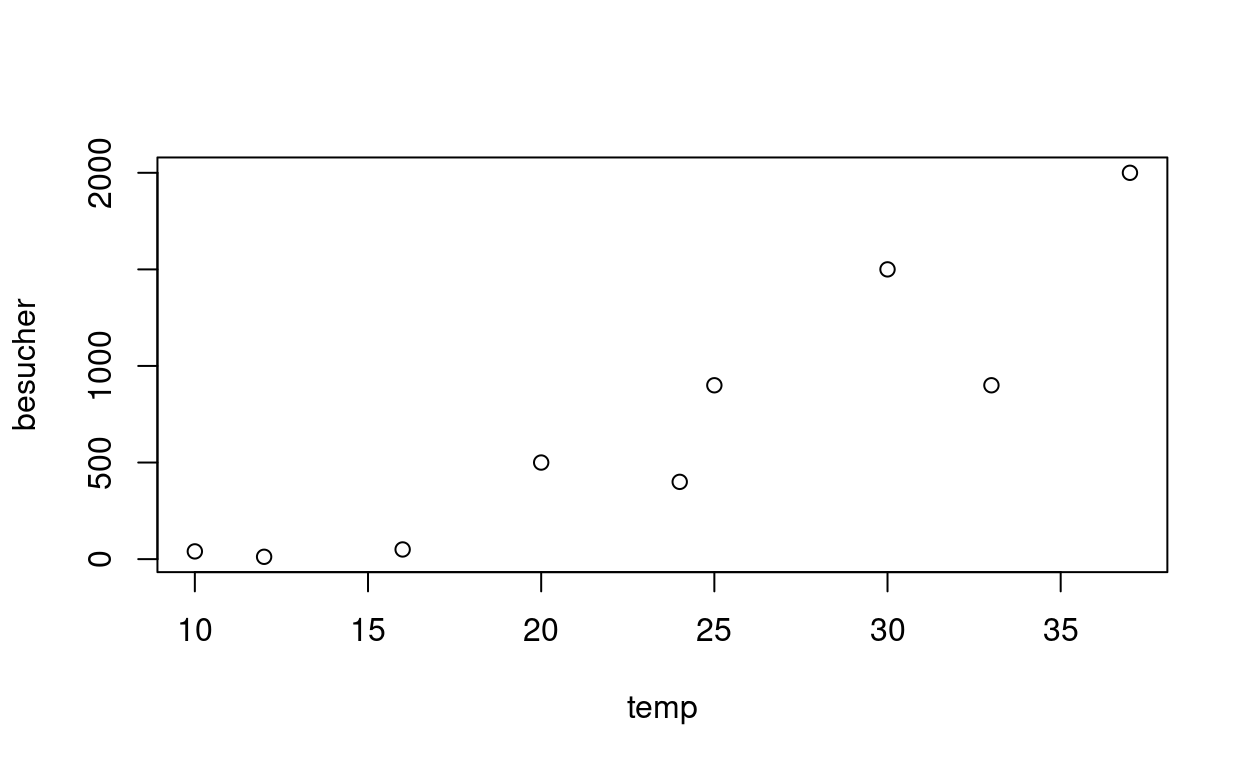
\includegraphics{solution_stat2.2_files/figure-latex/unnamed-chunk-2-1.pdf}

\begin{Shaded}
\begin{Highlighting}[]
\CommentTok{# definiert das Modell (vgl. Skript Statistik 2)}
\NormalTok{model <-}\StringTok{ }\KeywordTok{aov}\NormalTok{(tot_sold }\OperatorTok{~}\StringTok{ }\NormalTok{label_content, }\DataTypeTok{data =}\NormalTok{ df)}

\KeywordTok{summary.lm}\NormalTok{(model)}
\end{Highlighting}
\end{Shaded}

\begin{verbatim}
## 
## Call:
## aov(formula = tot_sold ~ label_content, data = df)
## 
## Residuals:
##      Min       1Q   Median       3Q      Max 
## -290.250 -135.083    1.667  125.500  282.417 
## 
## Coefficients:
##                           Estimate Std. Error t value Pr(>|t|)    
## (Intercept)                1135.58      48.92  23.211  < 2e-16 ***
## label_contentHot and Cold  -827.25      69.19 -11.956 1.54e-13 ***
## label_contentVegetarisch   -396.33      69.19  -5.728 2.15e-06 ***
## ---
## Signif. codes:  0 '***' 0.001 '**' 0.01 '*' 0.05 '.' 0.1 ' ' 1
## 
## Residual standard error: 169.5 on 33 degrees of freedom
## Multiple R-squared:  0.8125, Adjusted R-squared:  0.8012 
## F-statistic: 71.52 on 2 and 33 DF,  p-value: 1.007e-12
\end{verbatim}

\begin{Shaded}
\begin{Highlighting}[]
\CommentTok{# überprüft die Modelvoraussetzungen}
\KeywordTok{par}\NormalTok{(}\DataTypeTok{mfrow =} \KeywordTok{c}\NormalTok{(}\DecValTok{2}\NormalTok{,}\DecValTok{2}\NormalTok{))}
\KeywordTok{plot}\NormalTok{(model)}
\end{Highlighting}
\end{Shaded}

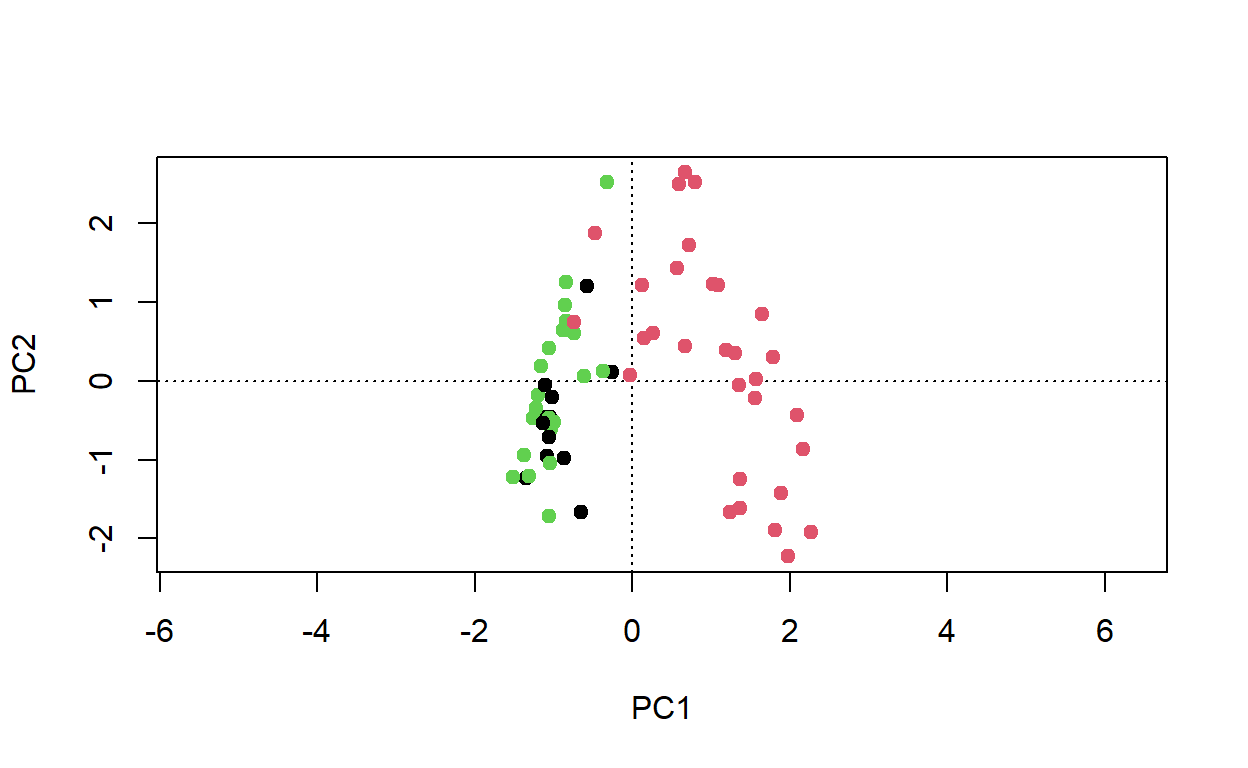
\includegraphics{solution_stat2.2_files/figure-latex/unnamed-chunk-2-2.pdf}
\\
\textbf{Fazit}: Inspektion der Modellvoraussetzung zeigt klare
Verletzungen des Residuelplots (zeigt einen ``Trichter'', siehe Skript
Statistik 2), somit Voraussetzung der Homoskedastizität verletzt.
Mögliche nächste Schritte:

\begin{itemize}
\tightlist
\item
  Menüinhalt ``Buffet'' aus der Analyse ausschliessen, da sowieso kein
  richtiger Menüinhalt (aber Informationsverlust)
\item
  Datentransformation z.B. log-Transformation
\item
  nicht-parametrischer Test (Achtung, auch dieser setzt Voraussetzungen
  voraus)
\item
  ein glm Model (general linear model) mit einer poisson/quasipoisson
  link Funktion (vgl. Skript Statistik 4), weitere Infos dazu
  \href{https://www.ncbi.nlm.nih.gov/pmc/articles/PMC5869353/}{Link} 
\end{itemize}

\begin{Shaded}
\begin{Highlighting}[]
\CommentTok{# überprüft die Voraussetzungen des Welch-Tests:}
\CommentTok{# Gibt es eine hohe Varianzheterogenität und ist die relative Verteilung der }
\CommentTok{# Residuen gegeben? (siehe Statistik 2)}
\CommentTok{# Ja Varianzheterogenität ist gegeben, aber die Verteilung der Residuen folgt }
\CommentTok{# einem "Trichter", also keiner "normalen/symmetrischen" Verteilung um 0}
\CommentTok{# Daher ziehe ich eine Transformation der AV einem nicht-parametrischen Test vor}
\CommentTok{# für weitere Infos: }
\CommentTok{# https://data.library.virginia.edu/interpreting-log-transformations-in-a-linear-model/}

\CommentTok{# achtung hier log10, bei Rücktransformation achten}
\NormalTok{model_log <-}\StringTok{ }\KeywordTok{aov}\NormalTok{(}\KeywordTok{log10}\NormalTok{(tot_sold) }\OperatorTok{~}\StringTok{ }\NormalTok{label_content, }\DataTypeTok{data =}\NormalTok{ df) }

\KeywordTok{par}\NormalTok{(}\DataTypeTok{mfrow =} \KeywordTok{c}\NormalTok{(}\DecValTok{2}\NormalTok{,}\DecValTok{2}\NormalTok{))}
\KeywordTok{plot}\NormalTok{(model_log) }\CommentTok{# scheint ok zu sein}
\end{Highlighting}
\end{Shaded}

\begin{verbatim}
## hat values (leverages) are all = 0.08333333
##  and there are no factor predictors; no plot no. 5
\end{verbatim}

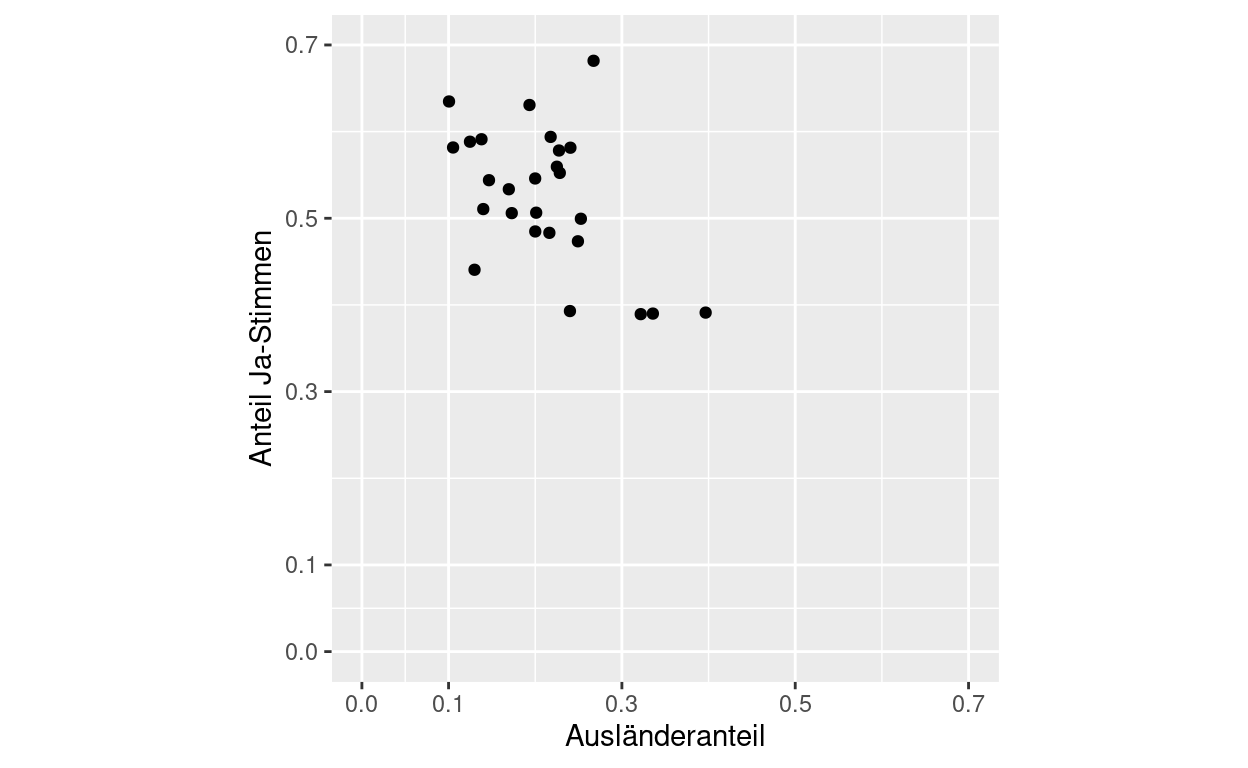
\includegraphics{solution_stat2.2_files/figure-latex/unnamed-chunk-3-1.pdf}

\begin{Shaded}
\begin{Highlighting}[]
\KeywordTok{summary.lm}\NormalTok{(model_log) }\CommentTok{# Referenzkategorie ist der Buffet-Inhalt}
\end{Highlighting}
\end{Shaded}

\begin{verbatim}
## 
## Call:
## aov(formula = log10(tot_sold) ~ label_content, data = df)
## 
## Residuals:
##       Min        1Q    Median        3Q       Max 
## -0.198920 -0.059343  0.003477  0.062579  0.150567 
## 
## Coefficients:
##                           Estimate Std. Error t value Pr(>|t|)    
## (Intercept)                3.04908    0.02585 117.942  < 2e-16 ***
## label_contentHot and Cold -0.56121    0.03656 -15.350  < 2e-16 ***
## label_contentVegetarisch  -0.19792    0.03656  -5.413 5.45e-06 ***
## ---
## Signif. codes:  0 '***' 0.001 '**' 0.01 '*' 0.05 '.' 0.1 ' ' 1
## 
## Residual standard error: 0.08956 on 33 degrees of freedom
## Multiple R-squared:  0.8802, Adjusted R-squared:  0.8729 
## F-statistic: 121.2 on 2 and 33 DF,  p-value: 6.238e-16
\end{verbatim}

\begin{Shaded}
\begin{Highlighting}[]
\KeywordTok{TukeyHSD}\NormalTok{(model_log) }\CommentTok{# (Statistik 2)}
\end{Highlighting}
\end{Shaded}

\begin{verbatim}
##   Tukey multiple comparisons of means
##     95% family-wise confidence level
## 
## Fit: aov(formula = log10(tot_sold) ~ label_content, data = df)
## 
## $label_content
##                                diff        lwr        upr   p adj
## Hot and Cold-Fleisch     -0.5612085 -0.6509215 -0.4714955 0.0e+00
## Vegetarisch-Fleisch      -0.1979175 -0.2876305 -0.1082044 1.6e-05
## Vegetarisch-Hot and Cold  0.3632910  0.2735780  0.4530041 0.0e+00
\end{verbatim}

\begin{Shaded}
\begin{Highlighting}[]
\CommentTok{# Achtung Beta-Werte resp. Koeffinzienten sind nicht direkt interpretierbar}
\CommentTok{# sie müssten zuerst wieder zurück transformiert werden, hier ein Beispiel dafür:}
\CommentTok{# für Buffet}
\DecValTok{10}\OperatorTok{^}\NormalTok{model_log}\OperatorTok{$}\NormalTok{coefficients[}\DecValTok{1}\NormalTok{]}
\end{Highlighting}
\end{Shaded}

\begin{verbatim}
## (Intercept) 
##    1119.655
\end{verbatim}

\begin{Shaded}
\begin{Highlighting}[]
\CommentTok{# für Fleisch}
\DecValTok{10}\OperatorTok{^}\NormalTok{(model_log}\OperatorTok{$}\NormalTok{coefficients[}\DecValTok{1}\NormalTok{] }\OperatorTok{+}\StringTok{ }\NormalTok{model_log}\OperatorTok{$}\NormalTok{coefficients[}\DecValTok{2}\NormalTok{])}
\end{Highlighting}
\end{Shaded}

\begin{verbatim}
## (Intercept) 
##    307.5216
\end{verbatim}

\begin{Shaded}
\begin{Highlighting}[]
\CommentTok{# für Vegi}
\DecValTok{10}\OperatorTok{^}\NormalTok{(model_log}\OperatorTok{$}\NormalTok{coefficients[}\DecValTok{1}\NormalTok{] }\OperatorTok{+}\StringTok{ }\NormalTok{model_log}\OperatorTok{$}\NormalTok{coefficients[}\DecValTok{3}\NormalTok{])}
\end{Highlighting}
\end{Shaded}

\begin{verbatim}
## (Intercept) 
##    709.8501
\end{verbatim}

\begin{center}\rule{0.5\linewidth}{0.5pt}\end{center}

\textbf{Methoden}

Ziel war es, die Unterschiede in den wöchentlichen Verkaufszahlen pro
Menüinhalt aufzuzeigen. Da die Responsevariable (Verkaufszahlen)
metrisch und die Prädiktorvariable kategorial sind, wurde eine
einfaktorielle ANOVA gerechnet. Die visuelle Inspektion des Modells
zeigte insbesondere schwere Verletzungen der Homoskedastizität. Der
Boxplot bestätigt dieser Befund. Weil die Voraussetzungen schwer
verletzt sind, wurde eine log-Transformation der Responsevariable
vorgenommen. Anschliessend wurde erneut eine ANOVA gerechnet und die
Modelvoraussetzungen visuell inspiziert: Homoskedastizität und
Normalverteilung der Residuen sind gegeben.

\begin{center}\rule{0.5\linewidth}{0.5pt}\end{center}

\textbf{Ergebnisse}

Die Menüinhalte (Fleisch, Vegetarisch und Buffet) unterscheiden sich in
den wöchentlichen Verkaufszahlen signifikant (F(2,15) = 121.22, p
\textless{} .001). Die Abbildung 1 zeigt die wöchentlichen
Verkaufszahlen pro Menüinhalt.

\begin{figure}
\centering
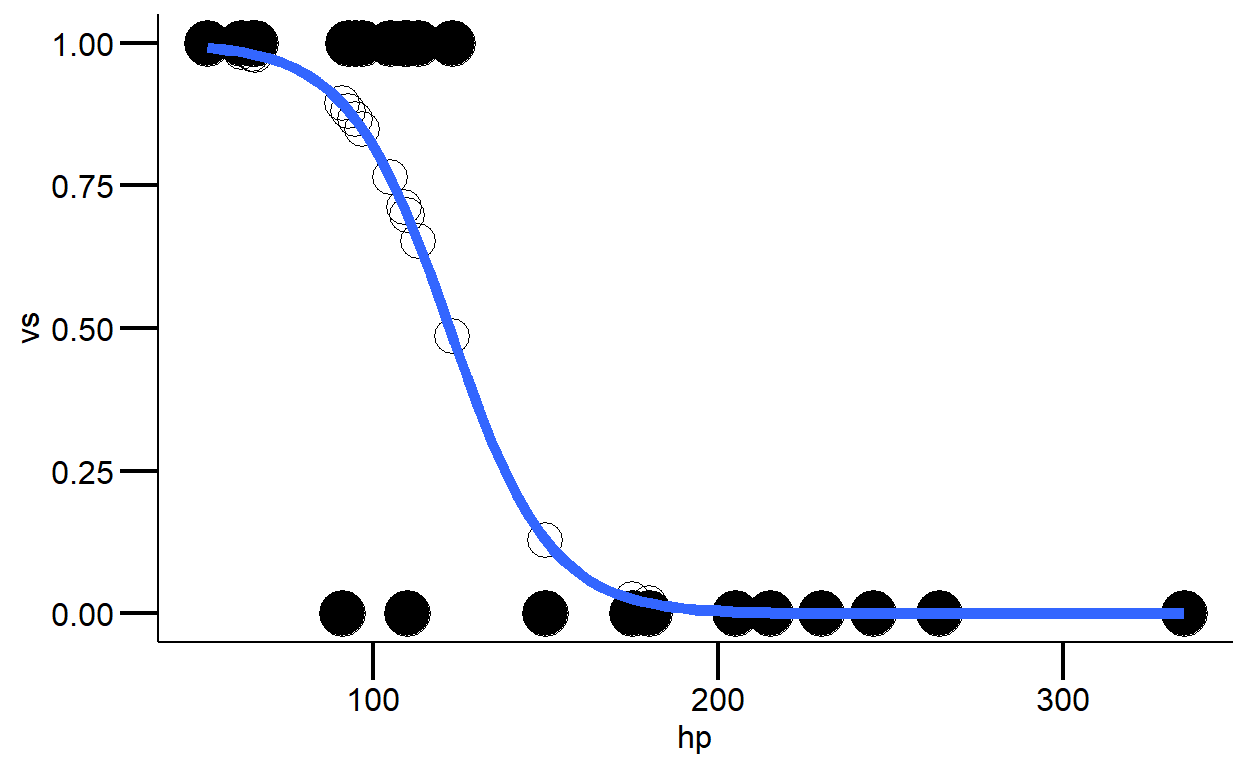
\includegraphics{solution_stat2.2_files/figure-latex/unnamed-chunk-4-1.pdf}
\caption{Die wöchentlichen Verkaufzahlen unterscheiden sich je nach
Menüinhalt stark. Das Modell wurde mit den log-tranformierten Daten
gerechnet.}
\end{figure}

\end{document}
